\documentclass[hyperref=unicode]{beamer}

\usepackage[absolute,overlay]{textpos}
\usepackage{graphicx}
\usepackage{adjustbox}
\usepackage{mhchem}
\usepackage{wrapfig}
\usepackage{multirow}
\adjustboxset*{center}
\usepackage[utf8]{inputenc}
\usepackage{caption}

%dělení slov
\usepackage{ragged2e}
\let\raggedright=\RaggedRight
%konec dělení slov

\usepackage{fontspec}
\usepackage{unicode-math}

\usepackage{polyglossia}
\setdefaultlanguage{czech}

\def\uv#1{„#1“}

\mode<presentation>{\usetheme{Madrid}}
\DefineNamedColor{named}{pozadi}{RGB}{200,200,200}
\usecolortheme{crane}

\setbeamertemplate{footline}[frame number]

\addtobeamertemplate{frametitle}{
   \let\insertframetitle\insertsectionhead}{}
\addtobeamertemplate{frametitle}{
   \let\insertframesubtitle\insertsubsectionhead}{}

\makeatletter
  \CheckCommand*\beamer@checkframetitle{\@ifnextchar\bgroup\beamer@inlineframetitle{}}
  \renewcommand*\beamer@checkframetitle{\global\let\beamer@frametitle\relax\@ifnextchar\bgroup\beamer@inlineframetitle{}}
\makeatother
\setbeamercolor{section in toc}{fg=blue}
\setbeamertemplate{section in toc shaded}[default][100]

\usepackage{tikz}
\usetikzlibrary{positioning}
\usetikzlibrary{arrows}
\usetikzlibrary{shapes.multipart}

\title[Crisis]
{Periodická tabulka  prvků}

\subtitle{Periodická tabulka prvků, periodicita prvků}

\author{Zdeněk Moravec, hugo@chemi.muni.cz \\ 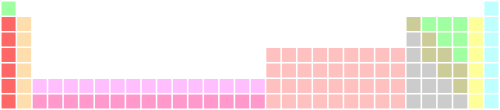
\includegraphics[keepaspectratio,width=8cm]{tableIntrod.png}}
\date{}

\begin{document}
\setbeamertemplate{caption}{\raggedright\insertcaption\par}
\setbeamerfont{caption}{size={\fontsize{5}{8}}}

\frame{\titlepage}

\section{Periodická tabulka prvků}
\frame{
	\frametitle{}
	\vfill
	\begin{itemize}
	\item Prvky jsou uspořádány podle vzrůstajícího atomového čísla.
	\item Jsou uspořádány do skupin a period.
	\item Ve \emph{skupinách} jsou prvky se stejným počtem valenčních elektronů. Díky podobné elektronové konfiguraci mají podobné chemické vlastnosti. Skupin je celkem 18.
	\item V \emph{periodách} jsou prvky jejichž valenční elektrony obsazují stejnou energetickou hladinu. Všechny dosud známé prvky jsou v periodách 1---7.
	\item Dále můžeme prvky rozdělit do čtyřech \emph{bloků}, podle typu orbitalu, který obsadil poslední elektron. Známe čtyři bloky - s, p, d a f.
	\item  Podle fyzikálních a chemických vlastností rozdělujeme prvky do tří velkých skupin --- kovy, polokovy a nekovy.
	\end{itemize}
	\vfill
}

\frame{
	\frametitle{}
	\vfill
	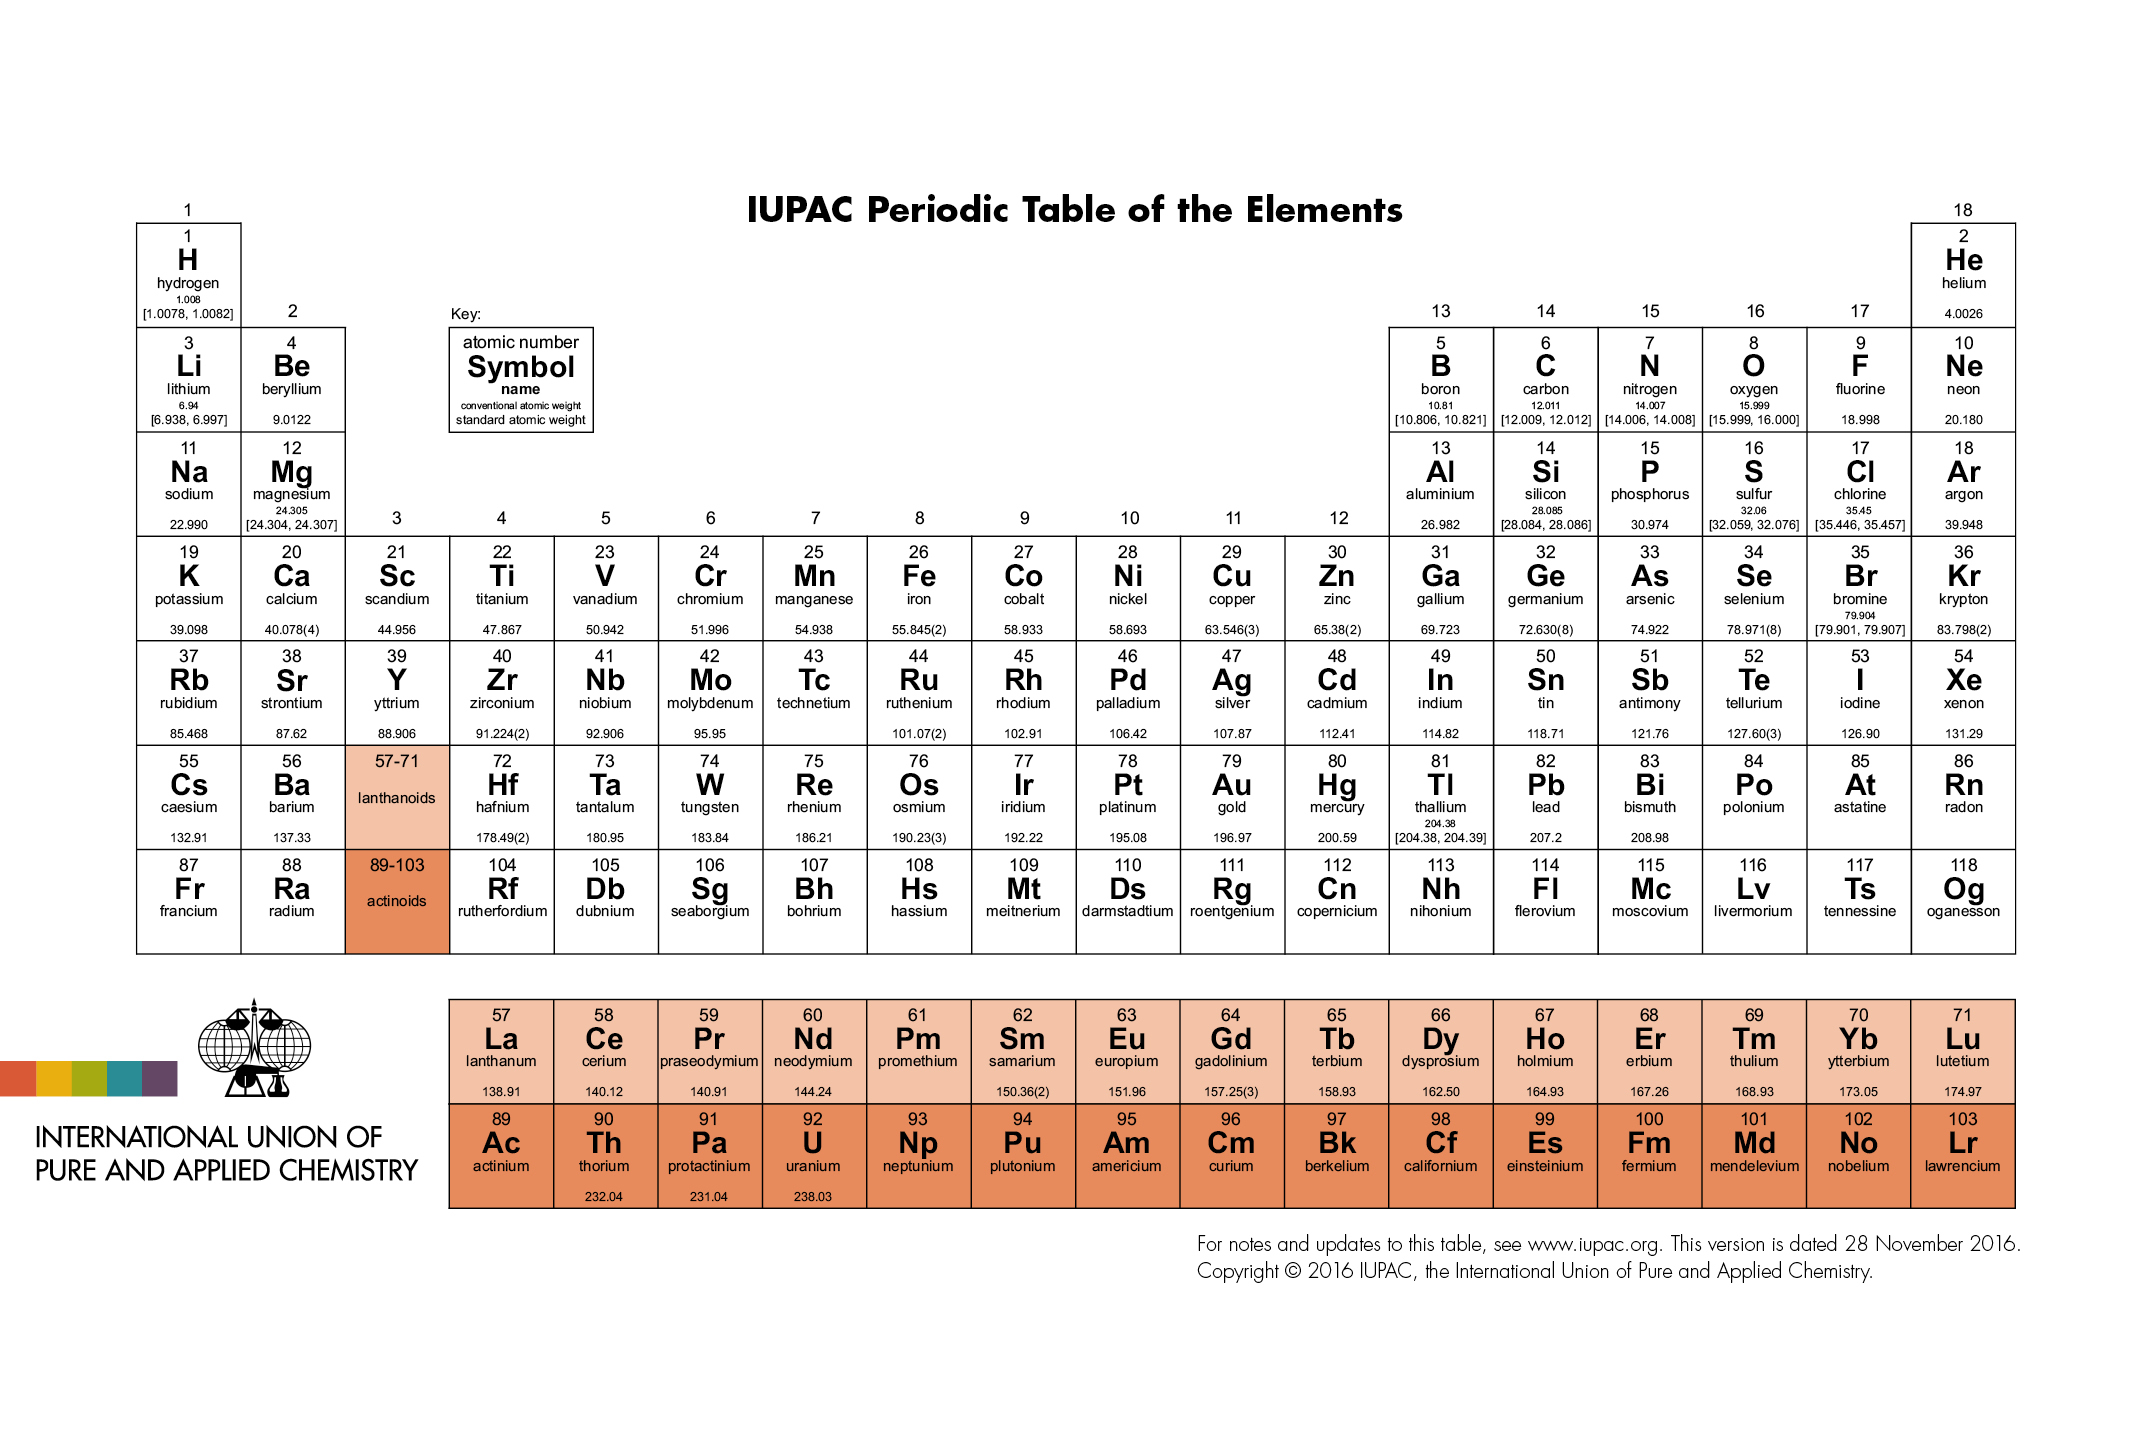
\includegraphics[keepaspectratio,width=\textwidth]{PSP.png}
	\vfill
}

\subsection{Nové prvky}
\frame{
	\frametitle{}
	\vfill
	\begin{tabular}{|c|c|c|c|}
		\hline
		\multicolumn{4}{|c|}{\textbf{Nové prvky 7. periody}}\\\hline
		\textbf{Protonové číslo} & \textbf{Symbol} & \textbf{Český název} & \textbf{Latinský název} \\\hline
		113 & Nh & Nihonium & Nihonium \\\hline
		114 & Fl & Flerovium & Flerovium \\\hline
		115 & Mc & Moskovium & Moscovium \\\hline
		116 & Lv & Livermorium & Livermorium \\\hline
		117 & Ts & Tennessin & Tennessine \\\hline
		118 & Og & Oganesson & Oganesson  \\\hline
	\end{tabular}
	\footnotetext[1]{\href{https://iupac.org/iupac-is-naming-the-four-new-elements-nihonium-moscovium-tennessine-and-oganesson/}{IUPAC IS NAMING THE FOUR NEW ELEMENTS NIHONIUM, MOSCOVIUM, TENNESSINE, AND OGANESSON}}
	\vfill
}


\subsection{Skupiny}
\frame{
	\frametitle{}
	\vfill
	\begin{itemize}
	\item 1. skupina (Alkalické kovy): \textbf{H}ana \textbf{Lí}bá \textbf{Na} \textbf{K}řižovatce \textbf{R}o\textbf{b}ustního \textbf{C}e\textbf{s}táře \textbf{Fr}antu
	\item 2. skupina (Kovy alkalických zemin): \textbf{Bě}žela \textbf{M}a\textbf{g}da \textbf{Ca}ňonem, \textbf{Sr}azila \textbf{Ba}nán \textbf{Ra}menem
	\item 13. skupina (Triely): \textbf{B}yl \textbf{Al}exej \textbf{Ga}garin \textbf{In}dickým \textbf{Tl}umočníkem?
	\item 14. skupina (Tetrely): \textbf{C}opak \textbf{Si} \textbf{Ge}rtruda \textbf{Sn}ědla \textbf{P}lom\textbf{b}u
	\item 15. skupina (Pentely): \textbf{N}áš \textbf{P}an \textbf{As}istent \textbf{Sb}írá \textbf{Bi}kiny
	\item 16. skupina (Chalkogeny): \textbf{Ó} \textbf{S}lečny \textbf{Se}jměte \textbf{Te}nké \textbf{Po}dkolenky
	\item 17. skupina (Halogeny): \textbf{F}ranta \textbf{Cl}oumal \textbf{Br}omem \textbf{J}ako \textbf{At}let
	\item 18. skupina (Inertní plyny): \textbf{He}lena \textbf{Ne}se \textbf{Ar}ašídy \textbf{Kr}áli \textbf{Xe}nonu \textbf{Rá}no
	\end{itemize}
	\vfill
}

%http://www.imaturita.cz/maturitni-otazky/chemie/periodicka-tabulka/397/
\section{Periodicita vlastností prvků}
\frame{
	\frametitle{}
	\vfill
	\begin{itemize}
	\item Vlastnosti prvků odpovídají umístění prvku v PSP. Podobnost prvků v rámci skupiny PSP je dána podobnou konfigurací valenční elektronové vrstvy.
	\item \textbf{Atomový poloměr} v periodě klesá s rostoucím protonovým číslem, je to dáno zvyšujícím se nábojem jádra, které pak silněji přitahuje elektrony zaplňující valenční slupku. V rámci skupiny roste se stoupajícím protonovým číslem.
	\item \textbf{Elektronegativita} v periodě narůstá, ve skupině postupně klesá.
	\item \textbf{Ionizační energie} klesá v rámci skupiny, v rámci periody roste.
	\item \textbf{Redoxní vlastnosti} v levé části tabulky jsou redukční činidla (H, Na, Ca, Mg) a v pravé oxidační (F, O, Cl).
	\item \textbf{Acidobazické vlastnosti} v levé části tabulky jsou zásadotvorné prvky (Na, K, Ca, Mg) a v pravé kyselinotvorné (F, Cl, S).
	\end{itemize}
	\vfill
}

\frame{
	\frametitle{}
	\vfill
	\begin{figure}
	\begin{center}
	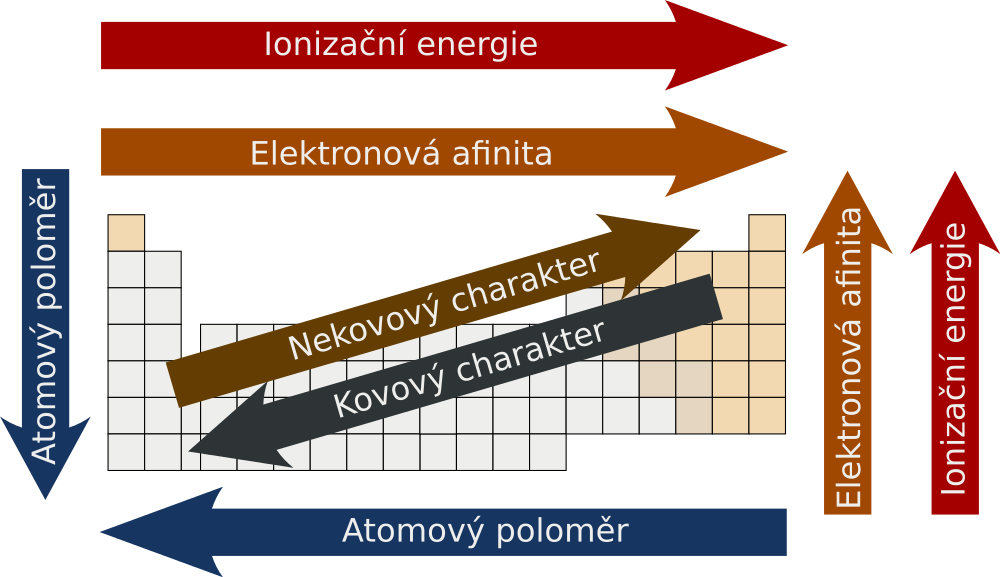
\includegraphics[keepaspectratio,width=110mm]{Periodicky_zakon.png}
	\caption{Autor: Mirek2. \url{https://commons.wikimedia.org/wiki/File:Periodicky_zakon.svg}}
	\end{center}
	\end{figure}
	\vfill
}

\subsection{Atomové poloměry}
\frame{
	\frametitle{}
	\vfill
	\begin{figure}
	\begin{center}
	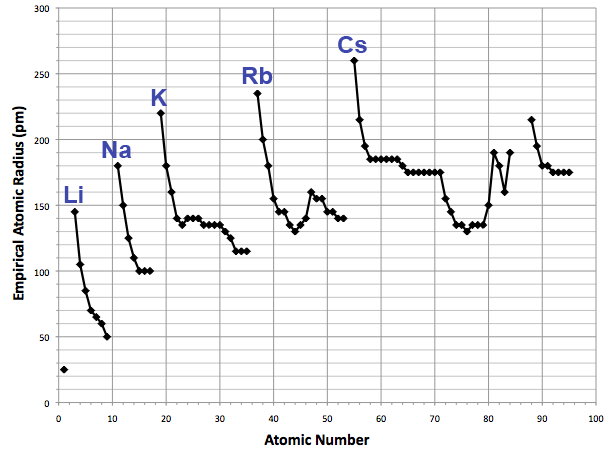
\includegraphics[keepaspectratio,width=90mm]{Empirical_atomic_radius_trends.png}
	\caption{Autor: StringTheory11. \url{https://commons.wikimedia.org/wiki/File:Empirical_atomic_radius_trends.png}}
	\end{center}
	\end{figure}
	\vfill
}

\subsection{Atomové a iontové poloměry}
\frame{
	\frametitle{}
	\vfill
	\begin{figure}
	\begin{center}
	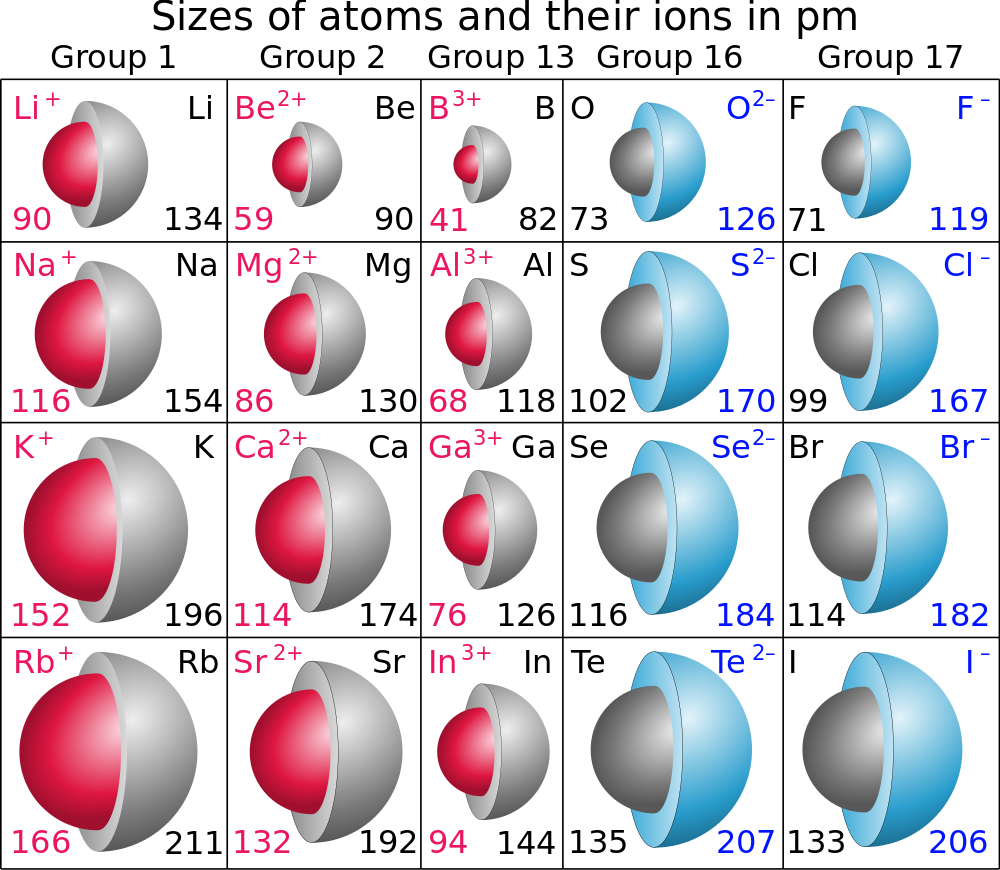
\includegraphics[keepaspectratio,width=80mm]{Atomic_and_ionic_radii.png}
	\caption{Autor: Popnose. \url{https://commons.wikimedia.org/wiki/File:Atomic & ionic radii.svg}}
	\end{center}
	\end{figure}
	\vfill
}

\subsection{První ionizační energie}
\frame{
	\frametitle{}
	\vfill
	\begin{figure}
	\begin{center}
	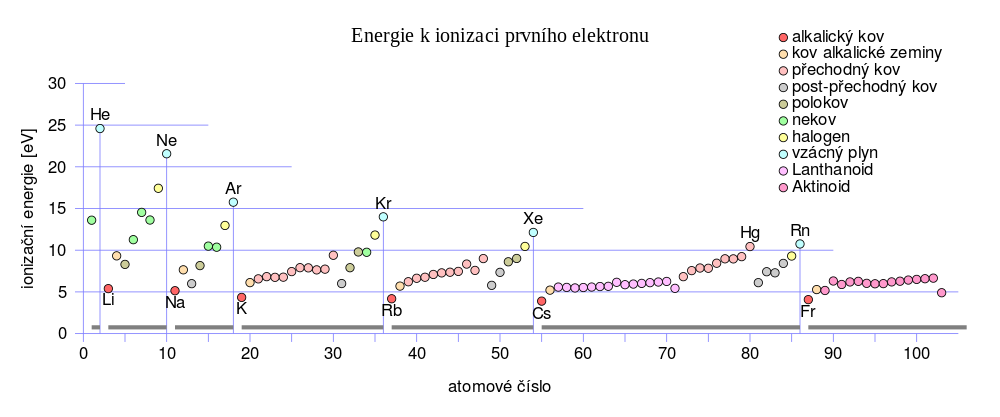
\includegraphics[keepaspectratio,width=120mm]{First_Ionization_Energy.png}
	\caption{Autor: Sponk. \url{https://commons.wikimedia.org/w/index.php?lang=cs&title=File:First_Ionization_Energy.svg}}
	\end{center}
	\end{figure}
	\vfill
}

\section{Literatura}
\frame{
	\frametitle{}
	\vfill
	\begin{itemize}
	\item KLIKORKA, Jiří a Jaroslav HOLEČEK. Obecná a anorganická chemie: určeno pro posl. Vys. školy chemicko-technologické v Pardubicích. 1. vyd. Praha: Státní nakladatelství technické literatury, 1971, s. 145-384.
	\item HOUSECROFT, Catherine E a A SHARPE. Anorganická chemie. Vyd. 1. Praha: Vysoká škola chemicko-technologická v Praze, 2014, xxx, 1119 s. ISBN 978-80-7080-872-6.
	\item \href{http://chemwiki.ucdavis.edu/Inorganic_Chemistry/Descriptive_Chemistry/Periodic_Trends_of_Elemental_Properties/Periodic_Trends}{Periodic Trends} na UCDavis Chemwiki
	\end{itemize}
	\vfill
}

\end{document}